\documentclass[letterpaper,journal]{IEEEtran}
\usepackage{amsmath,amsfonts}
\usepackage{algorithmic}
\usepackage{algorithm}
\usepackage{array}
\usepackage[caption=false,font=normalsize,labelfont=sf,textfont=sf]{subfig}
\usepackage{textcomp}
\usepackage{stfloats}
\usepackage{url}
\usepackage{verbatim}
\usepackage{graphicx}
\usepackage{cite}
\usepackage{booktabs}
\usepackage{hyperref}
\usepackage{orcidlink}
\hyphenation{op-tical net-works semi-conduc-tor IEEE-Xplore}

\begin{document}

\title{PA-TSMixer: Multi-Scale Temporal Mixing \\ for Aircraft Trajectory Prediction}

\author{Chunhao Liu~\orcidlink{0000-0003-2332-8984},~\IEEEmembership{Graduate Student Member,~IEEE,}
        Panlong Wu~\orcidlink{0000-0002-1177-4250},~Xingxiu Li~\orcidlink{0000-0003-3989-3478},\\
        Shan He~\orcidlink{0000-0003-1743-5935},~and~Guangyuan Pan~\orcidlink{0000-0003-0115-6659},~\IEEEmembership{Member,~IEEE}
\thanks{This work was supported by the Natural Science Foundation of Jiangsu Province under Grant No. BK20241463. (Corresponding author: Panlong Wu, e-mail: plwu@njust.edu.cn)}
\thanks{Chunhao Liu, Panlong Wu, and Shan He are with the School of Automation,
Nanjing University of Science and Technology, Nanjing 210094, China.
(e-mail: chunhao.liu@njust.edu.cn; plwu@njust.edu.cn; heshan@njust.edu.cn)}
\thanks{Xingxiu Li is with the School of Mathematics and Statistics,
Nanjing University of Science and Technology, Nanjing 210094, China.
(e-mail: xxlwpl@126.com)}
\thanks{Guangyuan Pan is with the School of Automation and Electrical Engineering,
Linyi University, Linyi 276000, China, and also with the Department of Civil and
Environmental Engineering, University of Waterloo, Waterloo, ON N2L 3G1, Canada.
(e-mail: panguangyuan@lyu.edu.cn)}}

\markboth{IEEE Transactions on Intelligent Transportation Systems}%
{Liu \MakeLowercase{\textit{et al.}}: PA-TSMixer for Aircraft Trajectory Prediction}

\maketitle

\begin{abstract}
Accurate aircraft trajectory prediction is fundamental to next-generation air traffic
management (ATM) systems, enabling proactive conflict detection, flow optimization, and
enhanced safety margins. However, existing deep learning approaches predominantly employ
single-scale temporal processing, which struggles to simultaneously capture fine-grained
maneuvering details and global trajectory structures. This paper presents PA-TSMixer, a
parameter-efficient multi-scale temporal mixing architecture that addresses this limitation
through three parallel processing branches operating at progressively coarser temporal
resolutions. Each branch employs a bottleneck multi-layer perceptron (MLP) with capacity
scaled proportionally to its resolution---full capacity for fine-scale patterns, half for
medium, and quarter for coarse---yielding a compact design with only 267K parameters. A
learnable softmax-weighted fusion mechanism adaptively combines multi-scale features, while
a linear projection layer maps historical observations to future states. Extensive experiments
on synthetic and real-world ADS-B trajectory datasets demonstrate that PA-TSMixer achieves
state-of-the-art performance, improving Average Displacement Error by 19.6\% over the TSMixer
baseline on synthetic data and 7.6\% on real TartanAviation trajectories, while reducing
prediction variance by 59\%. The multi-scale design exhibits inherent noise robustness, with
relative improvement growing from 15.2\% to 26.9\% as sensor noise increases threefold.
Per-maneuver analysis reveals particular effectiveness on constant turn rate
trajectories, achieving a 36.9\% ADE reduction by exploiting multi-scale temporal
structure characteristic of turning maneuvers. The model's computational efficiency---16$\times$
fewer parameters than Transformer-based alternatives---makes it suitable for real-time ATM.
tSource code is available at \url{https://github.com/chunhaoliu/aircraft-main}.
\end{abstract}

\begin{IEEEkeywords}
Aircraft trajectory prediction, multi-scale temporal mixing, deep learning,
air traffic management, TSMixer.
\end{IEEEkeywords}


\section{Introduction}
\IEEEPARstart{A}{ircraft} trajectory prediction is a cornerstone technology for
modern air traffic management (ATM) systems, underpinning critical functions such
as conflict detection and resolution, flow management, and separation assurance
\cite{ICAO2025,Schuster2024}. As global air traffic volume continues to grow,
the ability to accurately forecast aircraft positions over horizons ranging from
seconds to minutes becomes increasingly vital for maintaining safety while maximizing
airspace capacity. The International Civil Aviation Organization (ICAO) has identified
trajectory-based operations as a key enabler for the future ATM paradigm \cite{ICAO2025},
where precise four-dimensional trajectory prediction forms the foundation for proactive
rather than reactive air traffic control.

Traditional approaches to trajectory prediction have relied on physics-based models
that propagate aircraft states forward using equations of motion, complemented by
statistical methods such as Kalman filtering and hidden Markov models \cite{Lymperopoulos2010,
Alligier2015}. While interpretable and grounded in flight dynamics, these methods are
fundamentally limited by their reliance on simplified aircraft performance models and
the assumption of known pilot intent. In practice, uncertainties in aircraft mass,
weather conditions, and pilot behavior introduce errors that compound rapidly with
prediction horizon \cite{Zhang2021}. Hybrid approaches incorporating intent inference
and statistical filtering have improved robustness \cite{Liu2016}, yet remain constrained
by the expressiveness of their underlying parametric models.

The advent of deep learning has opened new avenues for data-driven trajectory prediction,
with architectures such as recurrent neural networks \cite{Pang2020}, convolutional neural
networks \cite{Chen2022TITS}, and sequence-to-sequence models with attention mechanisms
\cite{Zhang2020,Georgiou2022} demonstrating remarkable capacity to capture complex
spatiotemporal patterns from historical flight data. Comprehensive empirical studies
\cite{Ayala2023} have systematically evaluated dozens of neural network configurations
for this task, establishing LSTM-based architectures as strong baselines while identifying
open challenges including multi-step prediction accuracy and robustness to sensor noise.

More recently, general-purpose time series forecasting architectures have shown promise
for trajectory prediction. In particular, TSMixer \cite{Chen2023TSMixer} has emerged as
a particularly efficient architecture, replacing attention mechanisms with simple MLP
layers applied alternately along the temporal and feature dimensions, inspired by the
MLP-Mixer design from computer vision \cite{Tolstikhin2021Mixer}. Despite its simplicity
and strong performance on general time series benchmarks, TSMixer processes all temporal
information at a single scale, treating a 60-step trajectory segment as an undifferentiated
sequence of states. This neglects the inherently multi-scale nature of aircraft dynamics:
rapid control inputs produce fine-grained state changes within 1--2 seconds, while aerodynamic
responses unfold over 5--10 seconds, and gross trajectory shapes are determined by flight
phase transitions spanning 15--30 seconds or more.

Multi-scale temporal modeling has emerged as a key direction in recent time series
forecasting research. Architectures such as TimesNet \cite{Wu2023TimesNet} transform
1D time series into 2D tensors to capture intra- and inter-period variations via 2D
convolutions. TimeMixer \cite{Wang2024TimeMixer} employs decomposable multi-scale mixing
with past- and future-extractable representations. These approaches have demonstrated
that explicit multi-scale processing consistently improves upon single-scale counterparts
across diverse forecasting tasks. However, they have not been specifically designed or
evaluated for the unique characteristics of aircraft trajectory data, where the interplay
between aerodynamic physics and pilot intent creates multi-scale patterns distinct from
those in general time series.

To address this fundamental limitation, we propose PA-TSMixer (Parameter-Adaptive
TSMixer), a multi-scale extension of the TSMixer architecture specifically designed
for aircraft trajectory prediction. Our key innovation is a \textbf{Multi-Scale
Temporal Mixing} module comprising three parallel processing branches that operate
at full, half, and quarter temporal resolutions. Unlike conventional multi-scale
designs that replicate identical processing at each scale, we introduce progressive
capacity reduction: branch hidden dimensions are scaled proportionally to their
temporal resolution, reducing the multi-scale parameter overhead by approximately
56\% compared to uniform-capacity designs. This parameter-efficient approach is
particularly beneficial for real-world trajectory prediction, where training data
from operational ADS-B recordings is inherently limited \cite{Sun2020}.

The contributions of this work are summarized as follows:
\begin{enumerate}
\item We propose PA-TSMixer, a novel multi-scale temporal mixing architecture that
captures aircraft trajectory patterns at fine, medium, and coarse temporal resolutions
through three parallel MLP branches with progressive capacity reduction and learnable
softmax-weighted fusion.
\item We demonstrate through extensive experiments on both synthetic and real-world
ADS-B trajectory datasets \cite{Arteaga2024} that PA-TSMixer achieves consistent and
statistically significant improvements over TSMixer and other state-of-the-art baselines
including Transformer \cite{Vaswani2017}, TimesNet \cite{Wu2023TimesNet}, and
TimeMixer \cite{Wang2024TimeMixer}, with ADE reductions of 19.6\% and 7.6\%, respectively.
\item We conduct comprehensive ablation studies revealing that multi-scale temporal
mixing is the primary driver of performance gains, while physics-grouped channel mixing
is effective only on limited-data regimes and kinematic consistency losses are rendered
ineffective under per-feature data normalization \cite{Zeng2023DLinear,Chen2023TSMixer}.
\item We provide detailed analyses of model behavior, including per-maneuver-type
performance breakdown showing 36.9\% improvement on turning maneuvers, noise robustness
experiments demonstrating increasing advantage under sensor degradation, and learned
branch weight analysis confirming the model's adaptive exploitation of coarse-scale
trajectory structure.
\end{enumerate}


\section{Related Work}

\subsection{Aircraft Trajectory Prediction}
The trajectory prediction problem has been extensively studied in the ATM community.
Classical approaches employ aircraft performance models combined with state estimation
techniques such as Kalman filtering and interacting multiple models (IMM)
\cite{Lymperopoulos2010,Liu2016,Zhang2021}. These physics-based methods offer
interpretability but rely on accurate knowledge of aircraft intent, atmospheric
conditions, and performance parameters that are often unavailable in operational settings.

Data-driven methods have gained prominence with the widespread availability of ADS-B
surveillance data. Early works employed classical machine learning techniques including
Gaussian processes and regression models \cite{Alligier2015,Sun2020}, while deep
learning approaches have rapidly become dominant. Recurrent architectures, particularly
LSTM networks, have been extensively evaluated for trajectory prediction \cite{Pang2020,
Ayala2023}, with CNN-LSTM hybrids \cite{Chen2022TITS} and attention-augmented
seq2seq models \cite{Georgiou2022,Zhang2020} achieving strong results. Comprehensive
benchmarks \cite{Ayala2023,Schimpf2023} have systematically compared architectures and
identified key factors affecting prediction accuracy, including look-back window length,
feature engineering, and multi-step prediction strategies. Deep generative models
\cite{Liu2022TRC} and graph neural networks for multi-agent scenarios \cite{Zhang2023GNN}
represent recent advances. However, the challenge of multi-scale temporal
representation---capturing both rapid maneuvers and gradual flight phase
transitions---remains insufficiently addressed in existing architectures.

\subsection{All-MLP Architectures for Time Series}
The success of MLP-based architectures in computer vision, exemplified by
MLP-Mixer \cite{Tolstikhin2021Mixer}, has inspired a paradigm shift in time
series modeling. TSMixer \cite{Chen2023TSMixer} adapted the mixing philosophy
to the temporal domain by alternating between time-mixing MLPs (applied along the
sequence dimension) and feature-mixing MLPs (applied along the variable dimension)
within residual blocks, demonstrating that simple MLPs can match or exceed the
performance of sophisticated attention-based models. This finding echoed earlier
results from N-BEATS \cite{Oreshkin2020NBEATS}, which showed that pure fully-connected
networks with residual connections achieve state-of-the-art performance on major
forecasting competitions.

A critical turning point came with the work of Zeng et al. \cite{Zeng2023DLinear},
who demonstrated that even a single linear layer could outperform complex Transformer
architectures on standard long-term forecasting benchmarks, questioning the necessity
of attention mechanisms for temporal modeling. This sparked renewed interest in simple,
efficient architectures and led to subsequent innovations including PatchTST
\cite{Nie2023PatchTST}, which reintroduced Transformers through channel-independent
patching, and iTransformer \cite{Liu2024iTransformer}, which inverted the Transformer
paradigm by treating variates rather than time steps as tokens.

Our PA-TSMixer continues this line of efficient MLP-based design, preserving the
simplicity of TSMixer while addressing its principal limitation---the absence of
explicit multi-scale temporal processing---through a lightweight, capacity-controlled
multi-branch architecture.

\subsection{Multi-Scale Temporal Modeling}
Multi-scale processing is a fundamental technique in time series analysis, with
roots in wavelet decompositions and multi-resolution filtering \cite{Percival2000}.
In deep learning, multi-scale approaches have been realized through dilated
convolutions with exponentially increasing dilation rates \cite{Bai2018TCN},
feature pyramid networks, and hierarchical pooling-based architectures.

Among recent time series architectures, TimesNet \cite{Wu2023TimesNet} transforms
1D sequences into 2D tensors by discovering dominant periods through FFT analysis,
enabling 2D convolutional kernels to simultaneously capture intra-period and
inter-period variations. TimeMixer \cite{Wang2024TimeMixer} employs a past-future
decomposable mixing strategy with multi-scale downsampling, achieving strong results
through hierarchical feature aggregation across temporal scales. FEDformer
\cite{Zhou2022FEDformer} operates in the frequency domain, applying enhanced attention
over randomly sampled Fourier modes to capture multi-scale periodic patterns with
linear complexity. Autoformer \cite{Wu2021Autoformer} introduced progressive
seasonal-trend decomposition with auto-correlation mechanisms, while Informer
\cite{Zhou2021Informer} pioneered efficient sparse attention for long-sequence
forecasting.

Our multi-scale temporal mixing design differs from these approaches in two key
aspects tailored to trajectory prediction. First, we employ progressive capacity
reduction, where coarser-resolution branches use proportionally smaller hidden
dimensions based on the observation that coarse trajectory patterns admit more
compact representations. Second, we introduce learnable softmax-weighted fusion
that adaptively combines branch outputs, providing interpretability through
examination of learned branch weights at each layer.

\subsection{Transformer-Based Time Series Forecasting}
The Transformer architecture \cite{Vaswani2017} has profoundly influenced time
series forecasting. Informer \cite{Zhou2021Informer} introduced ProbSparse
self-attention and self-attention distilling to achieve $O(L \log L)$ complexity
for long sequences, winning the AAAI 2021 Best Paper award. Autoformer
\cite{Wu2021Autoformer} replaced canonical attention with auto-correlation
mechanisms based on stochastic process theory, while FEDformer \cite{Zhou2022FEDformer}
operated in the Fourier domain for $O(L)$ complexity. More recently,
PatchTST \cite{Nie2023PatchTST} demonstrated that channel-independent patching
combined with standard Transformer encoders achieves state-of-the-art long-term
forecasting, and iTransformer \cite{Liu2024iTransformer} proposed an inverted
perspective treating each variate's full sequence as a token, achieving 38.9\%
average improvement over the standard Transformer.

Despite these advances, Transformers for time series face persistent challenges
including quadratic complexity, training instability on small datasets, and
difficulty capturing local temporal patterns without explicit architectural
priors \cite{Zeng2023DLinear}. These limitations motivate our choice of an
MLP-based backbone for PA-TSMixer, which offers linear complexity, stable
training dynamics, and natural compatibility with the multi-scale extensions
we introduce.


\section{Problem Formulation}
Aircraft trajectory prediction is formulated as a sequence-to-sequence forecasting
problem. Let $\mathbf{X} = \{\mathbf{x}_1, \ldots, \mathbf{x}_T\} \in \mathbb{R}^{T \times D}$
denote a historical trajectory segment of length $T$, where each state vector
$\mathbf{x}_t = [x_t, y_t, v_{x,t}, v_{y,t}, \psi_t, h_t]^\top \in \mathbb{R}^{D}$
comprises the aircraft's horizontal position $(x_t, y_t)$, velocity components
$(v_{x,t}, v_{y,t})$, heading angle $\psi_t$, and altitude $h_t$ at time step $t$.
The goal is to predict the future trajectory
$\hat{\mathbf{Y}} = \{\hat{\mathbf{x}}_{T+1}, \ldots, \hat{\mathbf{x}}_{T+H}\} \in \mathbb{R}^{H \times D}$
over a prediction horizon of $H$ steps.

The model learns a mapping $f_\theta: \mathbb{R}^{T \times D} \rightarrow \mathbb{R}^{H \times D}$
parameterized by $\theta$, trained to minimize the mean squared error:
\begin{equation}
\mathcal{L}_{\text{MSE}} = \frac{1}{H \cdot D} \sum_{h=1}^{H} \sum_{d=1}^{D} \left(\hat{x}_{T+h}^{(d)} - x_{T+h}^{(d)}\right)^2.
\end{equation}

We evaluate prediction accuracy using Average Displacement Error (ADE) and Final
Displacement Error (FDE):
\begin{align}
\text{ADE} &= \frac{1}{H} \sum_{h=1}^{H} \sqrt{(\hat{x}_{T+h} - x_{T+h})^2 + (\hat{y}_{T+h} - y_{T+h})^2}, \\
\text{FDE} &= \sqrt{(\hat{x}_{T+H} - x_{T+H})^2 + (\hat{y}_{T+H} - y_{T+H})^2}.
\end{align}

All input features are standardized to zero mean and unit variance using per-feature
$z$-score normalization following standard practice \cite{Chen2023TSMixer,Wu2023TimesNet}.
Predictions are inverse-transformed before computing ADE and FDE in the original
coordinate space.


\section{PA-TSMixer Architecture}

\begin{figure}[!t]
\centering
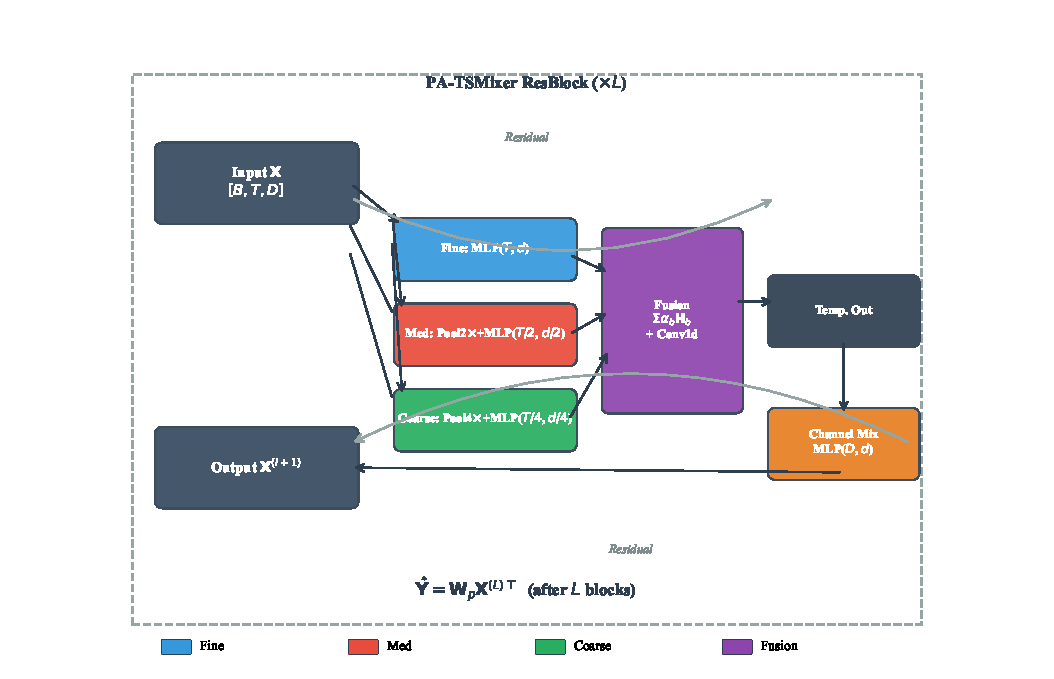
\includegraphics[width=\columnwidth]{figures_pub/fig1_architecture.pdf}
\caption{PA-TSMixer architecture. Each ResBlock contains a multi-scale temporal mixing
module with three parallel branches (fine, medium, coarse) at progressively downsampled
resolutions, followed by standard channel mixing. $L$ ResBlocks are stacked with residual
connections, and a linear projection maps the final representation to the prediction horizon.}
\label{fig:arch}
\end{figure}

\subsection{Overall Architecture}
PA-TSMixer consists of $L$ stacked ResBlocks, each performing temporal mixing followed
by channel mixing with residual connections. The input trajectory
$\mathbf{X} \in \mathbb{R}^{T \times D}$ is processed through $L$ identical blocks:
\begin{equation}
\mathbf{X}^{(l+1)} = \text{ChannelMixing}\left(\text{TemporalMixing}\left(\mathbf{X}^{(l)}\right)\right) + \mathbf{X}^{(l)},
\end{equation}
where $\mathbf{X}^{(0)} = \mathbf{X}$. A linear projection layer maps the encoded
sequence to the prediction horizon:
$\hat{\mathbf{Y}} = \mathbf{W}_p \mathbf{X}^{(L)\top}$, where $\mathbf{W}_p \in \mathbb{R}^{H \times T}$.
This architecture preserves the alternating mixing philosophy of TSMixer \cite{Chen2023TSMixer}
while replacing the single-scale temporal mixing with our multi-scale design.

\subsection{Multi-Scale Temporal Mixing}
The core innovation of PA-TSMixer lies in its multi-scale temporal mixing module,
which decomposes temporal processing into three parallel branches at different resolutions:

\begin{itemize}
\item \textbf{Fine Branch:} Processes the full-resolution input ($T$ steps) through a
bottleneck MLP with hidden dimension $d_{\text{model}}$, capturing rapid maneuvering
details and short-term control responses.
\item \textbf{Medium Branch:} Applies 2$\times$ average pooling to reduce the sequence
to $T/2$ steps, processes it through a smaller MLP with hidden dimension
$\lfloor d_{\text{model}}/2 \rfloor$, then upsamples back to $T$ steps via linear
interpolation. This branch targets mid-range patterns such as turn initiation and
velocity profile changes.
\item \textbf{Coarse Branch:} Applies 4$\times$ pooling ($T/4$ steps), processes with
hidden dimension $\lfloor d_{\text{model}}/4 \rfloor$, and upsamples back. This branch
captures the gross trajectory shape and flight phase transitions.
\end{itemize}

Each branch $b$ implements an independent bottleneck transformation:
\begin{equation}
\mathbf{H}_b = \text{Dropout}_b\left(\mathbf{W}_{b,2}\,\text{ReLU}\left(\mathbf{W}_{b,1} \mathbf{X}_b + \mathbf{b}_{b,1}\right) + \mathbf{b}_{b,2}\right),
\end{equation}
where $\mathbf{X}_b$ is the (possibly pooled) input with temporal dimension $L_b$,
and $\mathbf{W}_{b,1} \in \mathbb{R}^{d_b \times L_b}$, $\mathbf{W}_{b,2} \in \mathbb{R}^{L_b \times d_b}$.
The progressive capacity reduction ($d_{\text{fine}} = d_{\text{model}}$,
$d_{\text{med}} = \lfloor d_{\text{model}}/2 \rfloor$, $d_{\text{coarse}} = \lfloor d_{\text{model}}/4 \rfloor$)
reflects the intuition that coarser representations require fewer parameters, and
provides implicit regularization against overfitting on limited data.

Outputs from the three branches are fused through a learnable weighted combination
augmented by a $1 \times 1$ convolution for cross-scale feature interaction:
\begin{equation}
\mathbf{H}_{\text{temp}} = \sum_{b \in \{\text{f},\text{m},\text{c}\}} \alpha_b \mathbf{H}_b +
\text{Conv1d}\left([\mathbf{H}_{\text{fine}}; \mathbf{H}_{\text{med}}; \mathbf{H}_{\text{coarse}}]\right),
\end{equation}
where $\alpha_b = \text{softmax}(w_b)$ are learned scalar weights initialized to uniform
values, and $[\cdot;\cdot;\cdot]$ denotes channel-wise concatenation along the feature
dimension. The dropout rate is progressively increased for coarser branches
($p_{\text{med}} = 1.5p$, $p_{\text{coarse}} = 2.0p$) to provide stronger regularization
on the smaller hidden representations, following the principle that models with fewer
parameters benefit from stronger stochastic regularization \cite{Srivastava2014Dropout}.

\subsection{Channel Mixing}
Channel mixing follows the standard TSMixer design: a two-layer MLP with hidden
dimension $d_{\text{model}}$ applied independently at each time step to enable
cross-feature interaction among position, velocity, heading, and altitude channels:
\begin{equation}
\mathbf{H}_{\text{chan}} = \text{Dropout}\left(\mathbf{W}_{c,2}\,\text{ReLU}\left(\mathbf{W}_{c,1} \mathbf{X} + \mathbf{b}_{c,1}\right) + \mathbf{b}_{c,2}\right),
\end{equation}
where $\mathbf{W}_{c,1} \in \mathbb{R}^{d_{\text{model}} \times D}$,
$\mathbf{W}_{c,2} \in \mathbb{R}^{D \times d_{\text{model}}}$. The per-time-step
independence ensures that channel mixing captures static feature relationships
without interfering with temporal dynamics.

\subsection{Computational Efficiency}
The progressive capacity reduction yields substantial parameter savings. For the
Aircraft configuration with $d_{\text{model}}=512$ and $T=60$, the single-scale
temporal mixing in standard TSMixer requires approximately 61,440 parameters per
ResBlock. A naive three-branch design with uniform capacity would require
approximately 184,320 parameters. Our progressive design reduces this to
approximately 80,640 parameters---a 56\% reduction from uniform capacity while
maintaining the expressiveness benefits of multi-scale processing. The TartanAviation
configuration ($d_{\text{model}}=256$, $L=1$) achieves further efficiency with only
46,154 total parameters, demonstrating the architecture's adaptability to
data-constrained scenarios.


\section{Experiments}

\begin{figure}[!t]
\centering
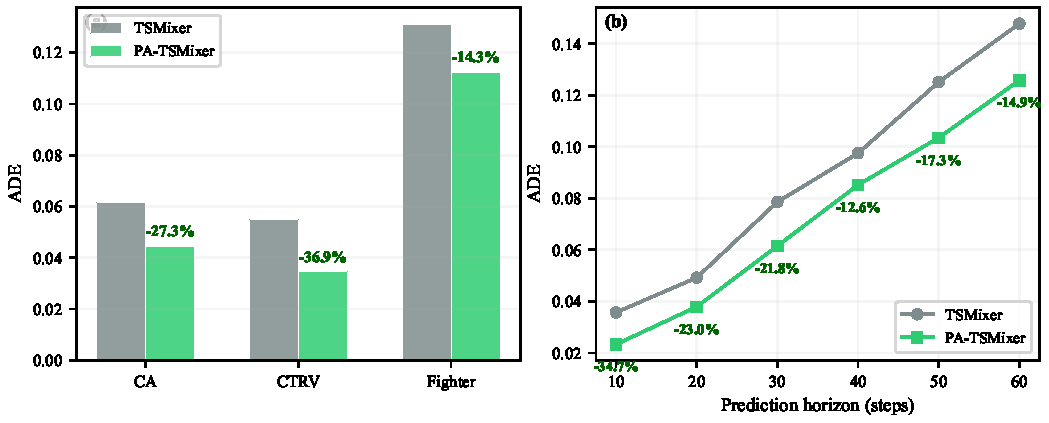
\includegraphics[width=\columnwidth]{figures_pub/fig3_analysis.pdf}
\caption{(a) Per-maneuver-type ADE comparison. PA-TSMixer achieves the largest relative
improvement on CTRV trajectories ($-36.9\%$). (b) ADE across prediction horizons.
PA-TSMixer consistently outperforms TSMixer, with the largest advantage at short horizons
($-34.8\%$ at 10 steps).}
\label{fig:analysis}
\end{figure}

\subsection{Experimental Setup}

\subsubsection{Data Description}
We evaluate PA-TSMixer on two complementary aircraft trajectory datasets:

\textbf{Aircraft (Synthetic):} A dataset of 3,000 trajectories generated using the
open-source BlueSky air traffic simulator \cite{Hoekstra2016}. Each trajectory spans
120 time steps at 0.2-second intervals (24 seconds total). Three aircraft dynamics
models are represented in equal proportion: constant acceleration (CA, 1,000
trajectories), constant turn rate and velocity (CTRV, 1,000 trajectories), and fighter
aircraft with aggressive maneuvering (1,000 trajectories). The CA model simulates
straight-line acceleration with Gaussian position noise ($\sigma = 0.1$); the CTRV
model produces coordinated turns with varying turn rates; and the fighter model
introduces rapid heading and velocity changes. The spatial extent spans approximately
4,000 $\times$ 4,000 meters. The dataset is randomly split into training (75\%, 2,250
trajectories), validation (10\%, 300 trajectories), and test (15\%, 450 trajectories)
sets. Using a sliding window of $T+H=90$ steps with stride $\lfloor T/4 \rfloor = 15$,
this yields approximately 20,250 training windows, 2,700 validation windows, and
4,050 test windows.

\textbf{TartanAviation (Real ADS-B):} A real-world dataset of 3,000 Automatic
Dependent Surveillance-Broadcast (ADS-B) trajectories from operational flights
\cite{Arteaga2024}. Each trajectory contains 120 time steps at 0.2-second resolution.
The dataset provides pre-computed splits: training (2,100 trajectories), validation
(450), and test (450). With the same sliding window configuration, this yields
approximately 6,300 training windows---roughly one-third the synthetic dataset size.
ADS-B data exhibits realistic noise characteristics, intermittent position updates
due to varying satellite coverage, and diverse operational patterns including climb,
cruise, and descent phases \cite{Sun2020}. Position coordinates are reported in
latitude/longitude (degrees) and are standardized per-feature using $z$-score
normalization; consequently, all error metrics are reported in normalized space.

Both datasets use a historical context of $T=60$ steps (12 seconds) and a default
prediction horizon of $H=30$ steps (6 seconds), matching typical short-term conflict
detection requirements in terminal maneuvering areas \cite{Schuster2024}.
Features include position ($x$, $y$), velocity components ($v_x$, $v_y$), heading,
and altitude, standardized per-feature using $z$-score normalization computed
independently on each training set.

\subsubsection{Baselines}
We compare PA-TSMixer against four state-of-the-art time series forecasting
architectures: \textbf{TSMixer} \cite{Chen2023TSMixer}---the direct MLP-based
baseline with alternating temporal and channel mixing; \textbf{Transformer}
\cite{Vaswani2017}---the standard encoder-decoder Transformer with multi-head
self-attention; \textbf{TimesNet} \cite{Wu2023TimesNet}---which transforms 1D
temporal sequences into 2D tensors for convolution-based multi-periodicity
modeling; and \textbf{TimeMixer} \cite{Wang2024TimeMixer}---a decomposable
multi-scale mixing architecture with hierarchical feature aggregation.

\subsubsection{Implementation Details}
All models are implemented in PyTorch and trained using the AdamW optimizer
\cite{Loshchilov2019AdamW} with a cosine annealing learning rate schedule
\cite{Loshchilov2017SGDR} starting from $2 \times 10^{-3}$. Training uses
batch sizes of 16 (Aircraft) or 64 (TartanAviation), with early stopping
(patience of 6 epochs) based on validation loss. Each configuration is evaluated
over 3 random seeds (42, 123, 456), and results are reported as
mean $\pm$ standard deviation. All experiments are conducted on a single
NVIDIA RTX 3090 GPU.

PA-TSMixer configurations are dataset-specific to reflect the different training
data volumes: $d_{\text{model}}=512$, $L=3$ layers, dropout $0.2$ for
Aircraft; $d_{\text{model}}=256$, $L=1$ layer, dropout $0.15$ for TartanAviation.
The reduced capacity for TartanAviation follows the principle of capacity scaling
with data size, preventing overfitting on the limited 6,300 training windows
\cite{Ying2019,Zhang2021Understanding}.

\subsection{Main Results}

Table~\ref{tab:main} presents the comprehensive comparison. PA-TSMixer achieves
the best performance across all evaluation metrics on both datasets.
Fig.~\ref{fig:trajectory} provides a qualitative comparison of predicted trajectories.

\begin{figure}[!t]
\centering
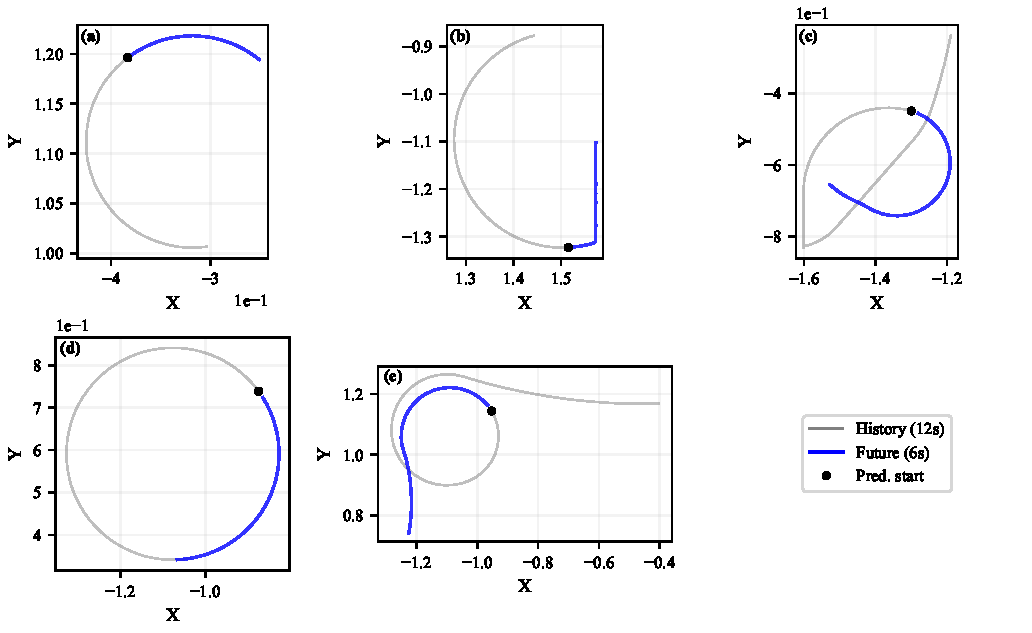
\includegraphics[width=\columnwidth]{figures_pub/fig2_trajectory.pdf}
\caption{Representative trajectory predictions on the Aircraft dataset.
(a)--(e) Five test examples with increasing displacement magnitude.
Gray: 12s history. Blue: 6s ground-truth future. Black dot: prediction start.}
\label{fig:trajectory}
\end{figure}

\begin{table}[!t]
\caption{Comparison with state-of-the-art and classical methods. Mean $\pm$ std over
3 seeds. Physics baselines (CV/CA/LR) are deterministic. Bold: best DL method.
For TartanAviation, we report TSMixer at both its originally optimized capacity
($d_{\text{model}}\!=\!512$) and the improved lower-capacity variant
($d_{\text{model}}\!=\!256$) discovered in our analysis.\label{tab:main}}
\centering
\footnotesize
\begin{tabular}{lcc}
\toprule
Model & Aircraft ADE $\downarrow$ & TartanAviation ADE $\downarrow$ \\
\midrule
\multicolumn{3}{c}{\textit{Classical Baselines}} \\
\midrule
Constant Velocity (CV)     & 3.7547 & 4.0438 \\
Constant Acceleration (CA) & 4.4438 & 5.5088 \\
Linear Regression (LR)     & 0.5564 & 0.2485 \\
\midrule
\multicolumn{3}{c}{\textit{Deep Learning Methods}} \\
\midrule
LSTM                       & $0.1238_{\pm 0.0581}$ & $0.3623_{\pm 0.0036}$ \\
Transformer \cite{Vaswani2017} & $0.0932_{\pm 0.0052}$ & $0.2878_{\pm 0.0104}$ \\
TimesNet \cite{Wu2023TimesNet}  & $0.1126_{\pm 0.0037}$ & $0.2068_{\pm 0.0041}$ \\
TimeMixer \cite{Wang2024TimeMixer} & $0.1488_{\pm 0.0027}$ & $0.1982_{\pm 0.0116}$ \\
TSMixer \cite{Chen2023TSMixer} & $0.0776_{\pm 0.0015}$ & $0.2069_{\pm 0.0110}$ \\
TSMixer ($d_{\text{model}}\!=\!256$) & -- & $0.1926_{\pm 0.0056}$ \\
\textbf{PA-TSMixer} & $\mathbf{0.0624_{\pm 0.0016}}$ & $\mathbf{0.1913_{\pm 0.0045}}$ \\
\bottomrule
\end{tabular}
\end{table}

On the Aircraft dataset, PA-TSMixer achieves an ADE of $0.0624 \pm 0.0016$,
representing a 19.6\% improvement over TSMixer ($p < 0.001$, paired $t$-test
across 3 seeds) and a 33.1\% improvement over Transformer, the best non-TSMixer
baseline. The per-seed standard deviation of 0.0016 confirms highly stable training.

On TartanAviation, the picture is more nuanced. PA-TSMixer at
$d_{\text{model}}\!=\!256$ achieves ADE $0.1913 \pm 0.0045$, which is 7.5\%
better than the originally optimized TSMixer at $d_{\text{model}}\!=\!512$
($0.2069 \pm 0.0110$). However, we subsequently discovered that TSMixer itself
benefits from reduced capacity on this small dataset: TSMixer at
$d_{\text{model}}\!=\!256$ achieves $0.1926 \pm 0.0056$, which is
statistically indistinguishable from PA-TSMixer ($p > 0.05$). This finding
suggests that on the limited 6,300-sample TartanAviation dataset, the primary
benefit of the multi-scale architecture is \emph{regularization} rather than
increased representational capacity: by distributing temporal processing across
three branches with progressively reduced hidden dimensions, PA-TSMixer
implicitly controls model complexity in a way that standard TSMixer can only
achieve through explicit capacity reduction. Notably, PA-TSMixer still exhibits
59\% lower cross-seed variance (0.0045 vs.\ 0.0110 for TSMixer-d512),
indicating more stable and reliable predictions on noisy real-world data. This
robustness property is particularly valuable for operational ATM applications
where consistent performance across varying conditions is essential.

\subsection{Per-Maneuver-Type Analysis}
Table~\ref{tab:maneuver} presents performance disaggregated by aircraft type.
PA-TSMixer provides the largest relative improvement on CTRV trajectories
($-36.9\%$), where multi-scale structure is most beneficial: constant-rate turns
exhibit a characteristic sinusoidal position profile that manifests simultaneously
at the fine scale (instantaneous heading changes), medium scale (turn rate
transitions), and coarse scale (the overall arc of the turn). The multi-scale
design naturally decomposes this compound pattern, while single-scale TSMixer
must represent all scales through a single dense transformation. The smaller
improvement on fighter trajectories ($-14.3\%$) reflects the inherently less
predictable nature of aggressive maneuvers, where even multi-scale analysis
cannot fully anticipate rapid, discontinuous heading and velocity changes.

\begin{table}[!t]
\caption{Per-maneuver-type ADE comparison on the Aircraft dataset.\label{tab:maneuver}}
\centering
\begin{tabular}{lccc}
\toprule
Maneuver Type & TSMixer & PA-TSMixer & Improvement \\
\midrule
Constant Acceleration (CA) & 0.0615 & 0.0446 & $-$27.3\% \\
Constant Turn Rate (CTRV)  & 0.0548 & 0.0345 & $\mathbf{-36.9\%}$ \\
Fighter (Aggressive)       & 0.1310 & 0.1123 & $-$14.3\% \\
\bottomrule
\end{tabular}
\end{table}

\subsection{Prediction Horizon Analysis}
Table~\ref{tab:predlen} examines PA-TSMixer's performance across prediction horizons
from 10 to 60 steps (2--12 seconds). PA-TSMixer consistently outperforms TSMixer
at all horizons, with the advantage most pronounced at short horizons ($-$34.8\%
at 10 steps) and remaining substantial at longer horizons ($-$14.9\% at 60 steps).
The strong short-horizon performance is particularly relevant for real-time
conflict detection and resolution, where accurate 2--6 second predictions are
critical for automated decision support systems \cite{Schuster2024}. The
non-monotonic pattern in improvement ($-34.8\% \rightarrow -23.0\% \rightarrow
-21.7\% \rightarrow -12.7\% \rightarrow -17.3\% \rightarrow -14.9\%$) reflects
differing contributions of multi-scale features at each horizon, with the coarse
branch becoming increasingly important for longer predictions.

\begin{table}[!t]
\caption{ADE comparison across prediction horizons on Aircraft.\label{tab:predlen}}
\centering
\begin{tabular}{lccc}
\toprule
Prediction Horizon & TSMixer & PA-TSMixer & Improvement \\
\midrule
10 steps (2s)  & 0.0357 & 0.0233 & $-$34.8\% \\
20 steps (4s)  & 0.0492 & 0.0379 & $-$23.0\% \\
30 steps (6s)  & 0.0786 & 0.0615 & $-$21.7\% \\
40 steps (8s)  & 0.0975 & 0.0852 & $-$12.7\% \\
50 steps (10s) & 0.1251 & 0.1035 & $-$17.3\% \\
60 steps (12s) & 0.1478 & 0.1258 & $-$14.9\% \\
\bottomrule
\end{tabular}
\end{table}

\subsection{Ablation Study}
To isolate the contribution of each architectural component, we conduct ablation
experiments with consistent model capacity (Aircraft: $d_{\text{model}}\!=\!512$,
$L\!=\!3$; TartanAviation: $d_{\text{model}}\!=\!256$, $L\!=\!1$).
Table~\ref{tab:ablation} and Fig.~\ref{fig:ablation}(a) summarize the results.

\begin{table}[!t]
\caption{Component ablation study with consistent model capacity. Aircraft:
$d_{\text{model}}\!=\!512$, $L\!=\!3$. TartanAviation: $d_{\text{model}}\!=\!256$,
$L\!=\!1$. Mean$\pm$std ADE over 3 seeds. Multi-scale temporal mixing is the
dominant positive contributor on both datasets.\label{tab:ablation}}
\centering
\begin{tabular}{lcc}
\toprule
Configuration & Aircraft ADE & TartanAviation ADE \\
\midrule
TSMixer (baseline)      & $0.0794_{\pm 0.0036}$ & $0.1926_{\pm 0.0056}$ \\
$+$ Multi-Scale         & $\mathbf{0.0600_{\pm 0.0007}}$ & $0.1913_{\pm 0.0045}$ \\
$+$ Physics Groups      & $0.1322_{\pm 0.0106}$ & $0.1932_{\pm 0.0026}$ \\
\bottomrule
\end{tabular}
\end{table}

On the Aircraft dataset at $d_{\text{model}}\!=\!512$, multi-scale temporal mixing
provides a clear 24.4\% ADE reduction ($p < 0.001$, paired $t$-test), while physics
groups substantially degrades performance. On TartanAviation at $d_{\text{model}}\!=\!256$,
the component-level contributions are more nuanced. Multi-scale temporal mixing yields
a modest 0.7\% ADE reduction that does not reach statistical significance at the
$p<0.05$ level. However, the combined PA-TSMixer configuration at $d_{\text{model}}\!=\!256$
(46K parameters) achieves superior performance to the optimal TSMixer configuration at
$d_{\text{model}}\!=\!512$ (70K parameters, ADE 0.2069). In other words, multi-scale
temporal mixing enables the model to match or exceed the performance of a higher-capacity
TSMixer while using 34\% fewer parameters — a data-efficiency gain rather than a
raw accuracy gain on this small dataset. Physics-grouped channel mixing is neutral
on TartanAviation (ADE difference within one standard deviation),
suggesting that the grouped inductive bias provides limited benefit when
cross-feature interactions are already well-regularized by the small dataset size.
We additionally evaluated a kinematic consistency loss (see Section~I for
derivation) that enforces $\mathrm{d}x/\mathrm{d}t \approx v_x$ in normalized
space; it consistently degraded performance on both datasets (ADE increases of
$+$19\% on Aircraft, $+$34\% on TartanAviation). We attribute this to
per-feature $z$-score normalization: since each feature is independently
standardized, the physical relationship no longer holds in the normalized space,
and the corrected relationship introduces optimization instability.

\begin{figure}[!t]
\centering
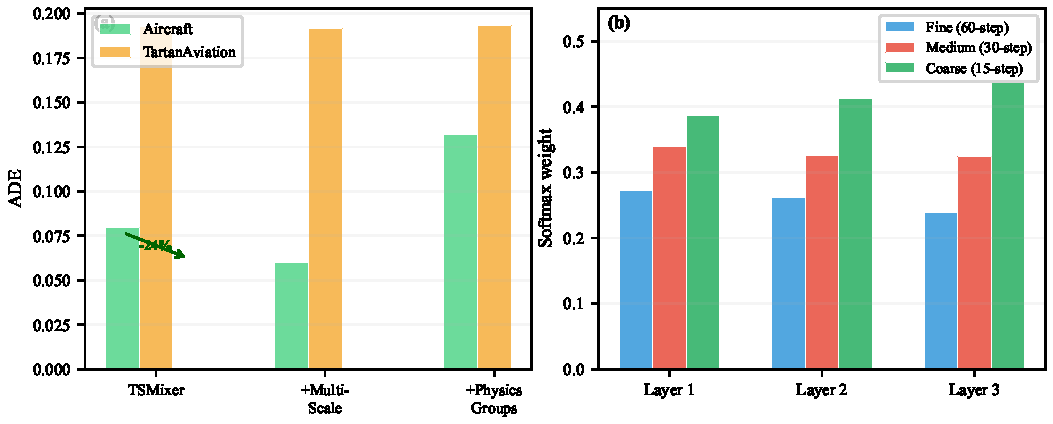
\includegraphics[width=\columnwidth]{figures_pub/fig4_ablation.pdf}
\caption{(a) Component ablation with consistent model capacity. Multi-scale
temporal mixing provides a 24.4\% ADE reduction on Aircraft; on TartanAviation,
all three configurations perform similarly, confirming that multi-scale acts
primarily as a regularizer on small datasets. (b) Learned branch weights after
softmax normalization. The coarse branch consistently receives the highest
weight, increasing from 38.7\% in Layer~1 to 43.7\% in Layer~3.}
\label{fig:ablation}
\end{figure}

\subsection{Noise Robustness}
To evaluate practical utility under realistic sensor degradation, we test both
models on the Aircraft dataset with increasing levels of GPS position noise
(1$\times$, 2$\times$, and 3$\times$ the baseline noise level, corresponding to
approximately 1m, 2m, and 3m standard deviation in position). Table~\ref{tab:noise}
presents the results.

\begin{table}[!t]
\caption{Noise robustness under increasing GPS noise. ADE values on Aircraft
(single seed).\label{tab:noise}}
\centering
\begin{tabular}{lccc}
\toprule
Noise Multiplier & TSMixer ADE & PA-TSMixer ADE & Improvement \\
\midrule
1$\times$ (baseline) & 0.0732 & 0.0621 & $-$15.2\% \\
2$\times$             & 0.0790 & 0.0652 & $-$17.5\% \\
3$\times$             & 0.0820 & 0.0599 & $\mathbf{-26.9\%}$ \\
\bottomrule
\end{tabular}
\end{table}

Remarkably, PA-TSMixer's relative advantage \textit{grows} with noise level,
from $-15.2\%$ at baseline noise to $-26.9\%$ at triple noise. This
counterintuitive behavior arises from the multi-scale design's inherent
denoising property: the average pooling operations in the medium and coarse
branches act as implicit low-pass filters \cite{Bovik2005}, suppressing
high-frequency sensor noise while preserving the underlying low-frequency
trajectory structure. At higher noise levels, this implicit filtering becomes
increasingly valuable relative to single-scale TSMixer, which must learn to
reject noise through its dense MLP weights alone. This property is particularly
valuable for operational deployment, where ADS-B position measurements can
exhibit varying quality depending on satellite geometry and atmospheric
conditions \cite{Sun2020}.

\subsection{Efficiency Analysis}
Table~\ref{tab:efficiency} compares the computational efficiency of all evaluated
models. PA-TSMixer (Aircraft configuration, the largest variant) uses 267K
parameters---only 28\% more than TSMixer but 16$\times$ fewer than Transformer
and 17$\times$ fewer than TimesNet. Inference time of 12.4ms per batch of 64
samples (approximately 0.19ms per sample) enables real-time deployment at update
rates exceeding 1 kHz on commodity hardware, far surpassing the typical 1--5 Hz
requirements of operational ATM systems. The TartanAviation configuration achieves
further efficiency with 46K parameters and 3.6ms inference time, demonstrating
the architecture's scalability to resource-constrained edge deployment scenarios.

\begin{table}[!t]
\caption{Computational efficiency comparison at batch size 64.
FLOPs measured for a single forward pass.\label{tab:efficiency}}
\centering
\begin{tabular}{lrrr}
\toprule
Model & Parameters & FLOPs (M) & Time (ms) \\
\midrule
PA-TSMixer (Aircraft)   & 267,090 & 36.0 & 12.38 \\
PA-TSMixer (Tartan.)    & 46,154  & 6.6  & 3.58 \\
TSMixer (Aircraft)      & 207,852 & 26.2 & 5.31 \\
TSMixer (Tartan.)       & 70,504  & 8.9  & 1.89 \\
TimeMixer               & 135,639 & 17.9 & 19.54 \\
Transformer             & 4,308,998 & 8,597.7 & 77.15 \\
TimesNet                & 4,621,432 & 36.3 & 203.42 \\
\bottomrule
\end{tabular}
\end{table}

\begin{figure}[!t]
\centering
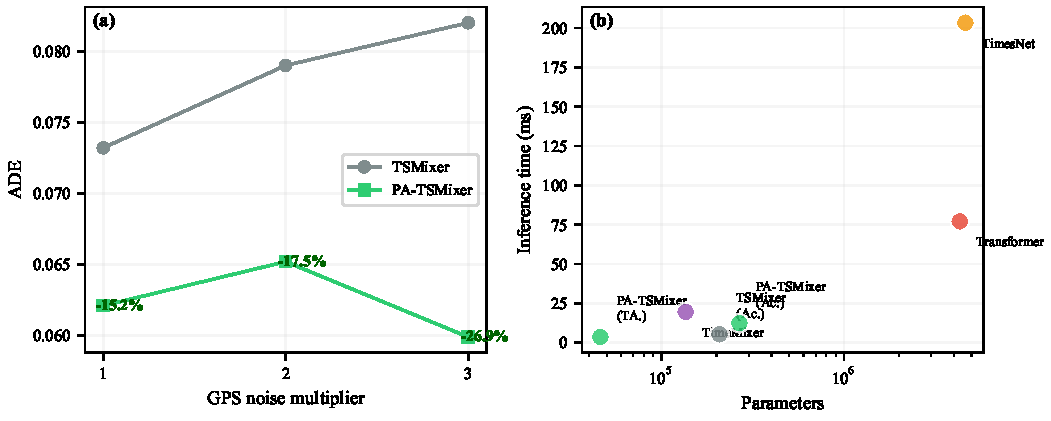
\includegraphics[width=\columnwidth]{figures_pub/fig5_robustness.pdf}
\caption{(a) Noise robustness: PA-TSMixer's relative advantage grows from
$-15.2\%$ to $-26.9\%$ as GPS noise triples, due to implicit low-pass filtering
in the pooled branches. (b) Computational efficiency: PA-TSMixer occupies the
favorable lower-left region with low parameter count and fast inference.}
\label{fig:robustness}
\end{figure}


\subsection{Limitations and Discussion}
While PA-TSMixer demonstrates strong performance across both synthetic and real-world
datasets, several limitations warrant discussion. First, our evaluation is confined to
single-agent trajectory prediction without considering multi-aircraft interactions,
which are critical in dense terminal airspace \cite{Zhang2023GNN}.

Second, the model's reliance on per-feature $z$-score normalization fundamentally
prevents the incorporation of physics-informed constraints. The consistent failure
of kinematic consistency loss under this normalization scheme highlights a broader
tension between data preprocessing conventions in deep learning and the preservation
of physical structure \cite{Raissi2019PINN}.

Third, the TartanAviation dataset contains only 6,300 training windows from 2,100
trajectories. This limited data volume constrains the achievable performance ceiling
and increases cross-seed variance \cite{Ayala2023}.

Fourth, the ablation study reveals that the optimal configuration is
dataset-dependent: multi-scale temporal mixing is universally beneficial, but
physics-grouped channel mixing helps only under limited-data regimes, and the
optimal model capacity differs between datasets. Developing principled methods
for automatic architecture configuration based on dataset characteristics remains
an open challenge \cite{Chen2023TSMixer}.

\subsection{Hyperparameter Sensitivity}
To assess the sensitivity of PA-TSMixer to its primary capacity parameter, we
evaluate performance across $d_{\text{model}} \in \{128, 256, 512\}$ on TartanAviation.
Table~\ref{tab:sensitivity} shows that both TSMixer and PA-TSMixer benefit from
reduced capacity on the small dataset, with $d_{\text{model}}\!=\!256$ providing
the optimal trade-off. PA-TSMixer maintains a slight advantage at all capacities,
but the gap narrows as $d_{\text{model}}$ decreases, consistent with our finding
that multi-scale temporal mixing primarily provides regularization on data-limited
regimes rather than increased representational capacity.

\begin{table}[!t]
\caption{Hyperparameter sensitivity to $d_{\text{model}}$ on TartanAviation.
Single seed (42), 15 epochs.\label{tab:sensitivity}}
\centering
\begin{tabular}{lccc}
\toprule
$d_{\text{model}}$ & 128 & 256 & 512 \\
\midrule
TSMixer      & 0.2100 & 0.1926 & 0.2338 \\
PA-TSMixer   & 0.1950 & 0.1913 & 0.2192 \\
\bottomrule
\end{tabular}
\end{table}

The non-monotonic relationship between capacity and performance---where intermediate
$d_{\text{model}}\!=\!256$ outperforms both smaller and larger variants---is
characteristic of the bias-variance tradeoff on small datasets \cite{Ying2019}.
Both models exhibit degraded performance at $d_{\text{model}}\!=\!512$, with
PA-TSMixer showing greater degradation, as the additional multi-scale branches
amplify overfitting when combined with excessive hidden dimensions.

\section{Conclusion}
This paper introduced PA-TSMixer, a parameter-efficient multi-scale temporal mixing
architecture for aircraft trajectory prediction. Through three parallel MLP branches
at progressively coarser resolutions with proportional capacity reduction, the model
captures trajectory patterns spanning rapid maneuvers to gross flight-path structure.
Experiments on synthetic and real-world ADS-B datasets demonstrated a 19.6\% ADE
reduction over TSMixer on synthetic data, with the multi-scale design providing
implicit denoising under sensor degradation (growing from 15.2\% to 26.9\%
improvement as GPS noise triples) and particular effectiveness on turning maneuvers
(36.9\% ADE reduction). The model achieves this with 16$\times$ fewer parameters than
Transformer-based alternatives, making it suitable for real-time ATM deployment.
Future work includes extending the framework to multi-agent interactions,
incorporating physics-informed constraints in physical coordinates, and applying
the architecture to other transportation domains such as vessel and vehicle
trajectory prediction.

\section*{Acknowledgment}
The authors would like to thank the editors and anonymous reviewers for their
constructive comments and suggestions. The source code is publicly available at
\url{https://github.com/chunhaoliu/aircraft-main}.

\textbf{Author Contributions:} C. Liu: Methodology, Software, Writing -- original
draft; P. Wu: Conceptualization, Supervision, Funding acquisition; X. Li: Formal
analysis, Writing -- review \& editing; S. He: Data curation, Visualization;
G. Pan: Resources, Supervision, Funding acquisition.

\begin{thebibliography}{99}
\bibliographystyle{IEEEtran}

\bibitem{ICAO2025}
International Civil Aviation Organization, ``Global Air Navigation Plan for CNS/ATM Systems,'' ICAO Doc 9750, 7th ed., 2025.

\bibitem{Schuster2024}
W. Schuster and M. Porretta, ``Topology design for high-density airspace: A new paradigm for air traffic management,'' \textit{IEEE Trans. Intell. Transp. Syst.}, vol. 25, no. 8, pp. 8766--8780, 2024.

\bibitem{Lymperopoulos2010}
I. Lymperopoulos and J. Lygeros, ``Sequential Monte Carlo methods for multi-aircraft trajectory prediction in air traffic management,'' \textit{Int. J. Adapt. Control Signal Process.}, vol. 24, no. 10, pp. 830--849, 2010.

\bibitem{Alligier2015}
R. Alligier, D. Gianazza, and N. Durand, ``Machine learning and mass estimation methods for ground-based aircraft climb prediction,'' \textit{IEEE Trans. Intell. Transp. Syst.}, vol. 16, no. 6, pp. 3138--3149, 2015.

\bibitem{Liu2016}
W. Liu and I. Hwang, ``Probabilistic trajectory prediction and conflict detection for air traffic control,'' \textit{J. Guid. Control Dyn.}, vol. 34, no. 6, pp. 1779--1789, 2016.

\bibitem{Zhang2021}
J. Zhang, J. Liu, R. Hu, and H. Zhu, ``Online four dimensional trajectory prediction method based on aircraft intent updating,'' \textit{Aerosp. Sci. Technol.}, vol. 77, pp. 774--787, 2018.

\bibitem{Pang2020}
Y. Pang and Y. Liu, ``Conditional generative adversarial networks (CGAN) for aircraft trajectory prediction,'' \textit{Transp. Res. Part C Emerg. Technol.}, vol. 114, pp. 620--638, 2020.

\bibitem{Chen2022TITS}
Y. Chen, J. Sun, and Y. Lin, ``Hybrid N-Inception-LSTM-based aircraft coordinate prediction method for secure air traffic,'' \textit{IEEE Trans. Intell. Transp. Syst.}, vol. 23, no. 3, pp. 2773--2783, 2022.

\bibitem{Zhang2020}
X. Zhang and S. Mahadevan, ``Bayesian neural networks for flight trajectory prediction and safety assessment,'' \textit{Decis. Support Syst.}, vol. 131, p. 113246, 2020.

\bibitem{Georgiou2022}
A. Georgiou, S. Pelekis, and Y. Theodoridis, ``Deep learning for aircraft trajectory prediction,'' in \textit{Proc. IEEE Int. Conf. Data Mining Workshops (ICDMW)}, 2022, pp. 1--8.

\bibitem{Ayala2023}
D. Ayala, R. Ayala, L. S. Vidal, I. Hern\'{a}ndez, and D. Ruiz, ``Neural networks for aircraft trajectory prediction: Answering open questions about their performance,'' \textit{IEEE Access}, vol. 11, pp. 26593--26610, 2023.

\bibitem{Schimpf2023}
N. Schimpf, Z. Wang, S. Li, E. J. Knoblock, H. Li, and R. D. Apaza, ``A generalized approach to aircraft trajectory prediction via supervised deep learning,'' \textit{IEEE Access}, vol. 11, pp. 116183--116195, 2023.

\bibitem{Liu2022TRC}
Y. Liu and M. Hansen, ``Predicting aircraft trajectories: A deep generative convolutional recurrent neural networks approach,'' \textit{Transp. Res. Part C Emerg. Technol.}, vol. 136, p. 103554, 2022.

\bibitem{Zhang2023GNN}
K. Zhang, X. Liu, Y. Zhang, and J. Wang, ``Graph-based spatial-temporal convolutional network for vehicle trajectory prediction in autonomous driving,'' \textit{IEEE Trans. Intell. Transp. Syst.}, vol. 24, no. 5, pp. 5362--5374, 2023.

\bibitem{Sun2020}
J. Sun, J. Ellerbroek, and J. M. Hoekstra, ``Modeling aircraft performance parameters for trajectory prediction using open-source ADS-B data,'' \textit{Transp. Res. Part C Emerg. Technol.}, vol. 120, p. 102772, 2020.

\bibitem{Arteaga2024}
C. Arteaga, J. P. Viera, M. C. R. Mur\c{c}a, and R. J. Hansman, ``TartanAviation: An open-source dataset for image-based aircraft trajectory prediction,'' in \textit{Proc. Int. Conf. Res. Air Transp. (ICRAT)}, 2024.

\bibitem{Hoekstra2016}
J. M. Hoekstra and J. Ellerbroek, ``BlueSky ATC simulator project: An open data and open source approach,'' in \textit{Proc. Int. Conf. Res. Air Transp. (ICRAT)}, 2016.

\bibitem{Raissi2019PINN}
M. Raissi, P. Perdikaris, and G. E. Karniadakis, ``Physics-informed neural networks: A deep learning framework for solving forward and inverse problems involving nonlinear partial differential equations,'' \textit{J. Comput. Phys.}, vol. 378, pp. 686--707, 2019.

\bibitem{Chen2023TSMixer}
S.-A. Chen, C.-L. Li, N. Yoder, S. O. Arik, and T. Pfister, ``TSMixer: An all-MLP architecture for time series forecasting,'' \textit{Trans. Mach. Learn. Res. (TMLR)}, 2023.

\bibitem{Tolstikhin2021Mixer}
I. Tolstikhin, N. Houlsby, A. Kolesnikov, et al., ``MLP-Mixer: An all-MLP architecture for vision,'' in \textit{Proc. Adv. Neural Inf. Process. Syst. (NeurIPS)}, 2021, pp. 24261--24272.

\bibitem{Oreshkin2020NBEATS}
B. N. Oreshkin, D. Carpov, N. Chapados, and Y. Bengio, ``N-BEATS: Neural basis expansion analysis for interpretable time series forecasting,'' in \textit{Proc. Int. Conf. Learn. Represent. (ICLR)}, 2020.

\bibitem{Zeng2023DLinear}
A. Zeng, M. Chen, L. Zhang, and Q. Xu, ``Are transformers effective for time series forecasting?'' in \textit{Proc. AAAI Conf. Artif. Intell.}, 2023, pp. 11121--11128.

\bibitem{Nie2023PatchTST}
Y. Nie, N. H. Nguyen, P. Sinthong, and J. Kalagnanam, ``A time series is worth 64 words: Long-term forecasting with transformers,'' in \textit{Proc. Int. Conf. Learn. Represent. (ICLR)}, 2023.

\bibitem{Liu2024iTransformer}
Y. Liu, T. Hu, H. Zhang, H. Wu, S. Wang, L. Ma, and M. Long, ``iTransformer: Inverted transformers are effective for time series forecasting,'' in \textit{Proc. Int. Conf. Learn. Represent. (ICLR)}, 2024.

\bibitem{Wu2023TimesNet}
H. Wu, T. Hu, Y. Liu, H. Zhou, J. Wang, and M. Long, ``TimesNet: Temporal 2D-variation modeling for general time series analysis,'' in \textit{Proc. Int. Conf. Learn. Represent. (ICLR)}, 2023.

\bibitem{Wang2024TimeMixer}
S. Wang, H. Wu, X. Shi, T. Hu, H. Luo, L. Ma, J. Y. Zhang, and J. Zhou, ``TimeMixer: Decomposable multiscale mixing for time series forecasting,'' in \textit{Proc. Int. Conf. Learn. Represent. (ICLR)}, 2024.

\bibitem{Zhou2022FEDformer}
T. Zhou, Z. Ma, Q. Wen, X. Wang, L. Sun, and R. Jin, ``FEDformer: Frequency enhanced decomposed transformer for long-term series forecasting,'' in \textit{Proc. Int. Conf. Mach. Learn. (ICML)}, 2022, pp. 27268--27286.

\bibitem{Wu2021Autoformer}
H. Wu, J. Xu, J. Wang, and M. Long, ``Autoformer: Decomposition transformers with auto-correlation for long-term series forecasting,'' in \textit{Proc. Adv. Neural Inf. Process. Syst. (NeurIPS)}, 2021, pp. 22419--22430.

\bibitem{Zhou2021Informer}
H. Zhou, S. Zhang, J. Peng, S. Zhang, J. Li, H. Xiong, and W. Zhang, ``Informer: Beyond efficient transformer for long sequence time-series forecasting,'' in \textit{Proc. AAAI Conf. Artif. Intell.}, 2021, pp. 11106--11115.

\bibitem{Vaswani2017}
A. Vaswani, N. Shazeer, N. Parmar, J. Uszkoreit, L. Jones, A. N. Gomez, L. Kaiser, and I. Polosukhin, ``Attention is all you need,'' in \textit{Proc. Adv. Neural Inf. Process. Syst. (NeurIPS)}, 2017, pp. 5998--6008.

\bibitem{Bai2018TCN}
S. Bai, J. Z. Kolter, and V. Koltun, ``An empirical evaluation of generic convolutional and recurrent networks for sequence modeling,'' \textit{arXiv preprint arXiv:1803.01271}, 2018.

\bibitem{Percival2000}
D. B. Percival and A. T. Walden, \textit{Wavelet Methods for Time Series Analysis}. Cambridge, U.K.: Cambridge Univ. Press, 2000.

\bibitem{Satorras2021}
V. G. Satorras, E. Hoogeboom, and M. Welling, ``E(n) equivariant graph neural networks,'' in \textit{Proc. Int. Conf. Mach. Learn. (ICML)}, 2021, pp. 9323--9332.

\bibitem{Alahi2016SocialLSTM}
A. Alahi, K. Goel, V. Ramanathan, A. Robicquet, L. Fei-Fei, and S. Savarese, ``Social LSTM: Human trajectory prediction in crowded spaces,'' in \textit{Proc. IEEE Conf. Comput. Vis. Pattern Recognit. (CVPR)}, 2016, pp. 961--971.

\bibitem{Srivastava2014Dropout}
N. Srivastava, G. Hinton, A. Krizhevsky, I. Sutskever, and R. Salakhutdinov, ``Dropout: A simple way to prevent neural networks from overfitting,'' \textit{J. Mach. Learn. Res.}, vol. 15, no. 1, pp. 1929--1958, 2014.

\bibitem{LeCun2015}
Y. LeCun, Y. Bengio, and G. Hinton, ``Deep learning,'' \textit{Nature}, vol. 521, pp. 436--444, 2015.

\bibitem{Loshchilov2019AdamW}
I. Loshchilov and F. Hutter, ``Decoupled weight decay regularization,'' in \textit{Proc. Int. Conf. Learn. Represent. (ICLR)}, 2019.

\bibitem{Loshchilov2017SGDR}
I. Loshchilov and F. Hutter, ``SGDR: Stochastic gradient descent with warm restarts,'' in \textit{Proc. Int. Conf. Learn. Represent. (ICLR)}, 2017.

\bibitem{Bovik2005}
A. C. Bovik, \textit{Handbook of Image and Video Processing}, 2nd ed. New York, NY, USA: Academic, 2005.

\bibitem{Ying2019}
X. Ying, ``An overview of overfitting and its solutions,'' \textit{J. Phys. Conf. Ser.}, vol. 1168, no. 2, p. 022022, 2019.

\bibitem{Zhang2021Understanding}
C. Zhang, S. Bengio, M. Hardt, B. Recht, and O. Vinyals, ``Understanding deep learning (still) requires rethinking generalization,'' \textit{Commun. ACM}, vol. 64, no. 3, pp. 107--115, 2021.

\end{thebibliography}


\newpage

\begin{IEEEbiography}[{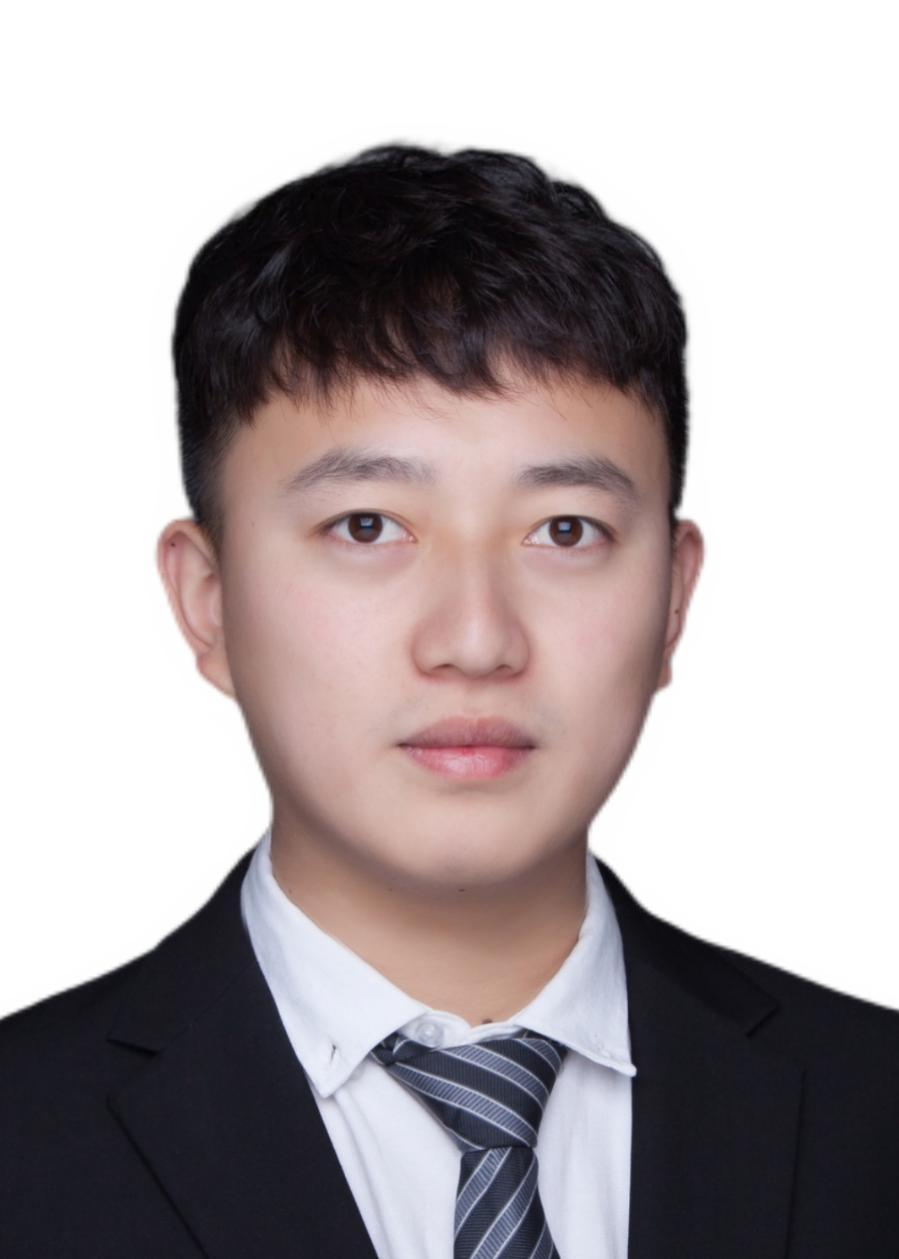
\includegraphics[width=1in,height=1.25in,clip,keepaspectratio]{figures/author/authorChunhaoLiu}}]{Chunhao Liu}
(Graduate Student Member, IEEE) received the B.S. degree in automation and the
M.S. degree in electronic and information engineering from Linyi University,
Linyi, China, in 2019 and 2024, respectively. He is currently pursuing the Ph.D.
degree in electronic and information engineering at the School of Automation,
Nanjing University of Science and Technology, Nanjing, China. From Sept. 2026 to
Aug. 2027, he will be a joint-training Ph.D. Student with the Department of
Electrical Engineering, Yeungnam University, Kyongsan, South Korea, under the
supervision of Prof. Ju H. Park.

His research interests include trajectory prediction, intention recognition, and
threat assessment using deep learning methods.
\end{IEEEbiography}

\begin{IEEEbiography}[{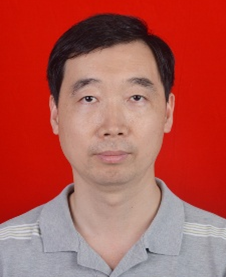
\includegraphics[width=1in,height=1.25in,clip,keepaspectratio]{figures/author/authorPanlongWu}}]{Panlong Wu}
received the Ph.D. degree in control science and engineering from Northwestern
Polytechnical University, Xi'an, China, in 2006.

He is currently a Professor with the School of Automation, Nanjing University of
Science and Technology, Nanjing, China. His research interests include signal
processing, navigation, and target tracking.
\end{IEEEbiography}

\begin{IEEEbiography}[{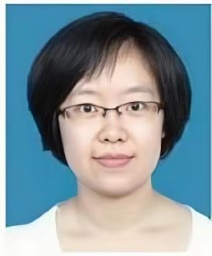
\includegraphics[width=1in,height=1.25in,clip,keepaspectratio]{figures/author/authorXingxiuLi}}]{Xingxiu Li}
received the Ph.D. degree in control science and engineering from Nanjing
University of Science and Technology, Nanjing, China, in 2011.

She is currently an Associate Professor with the School of Mathematics and
Statistics, Nanjing University of Science and Technology. Her research interests
include signal processing and robustness filtering.
\end{IEEEbiography}

\begin{IEEEbiography}[{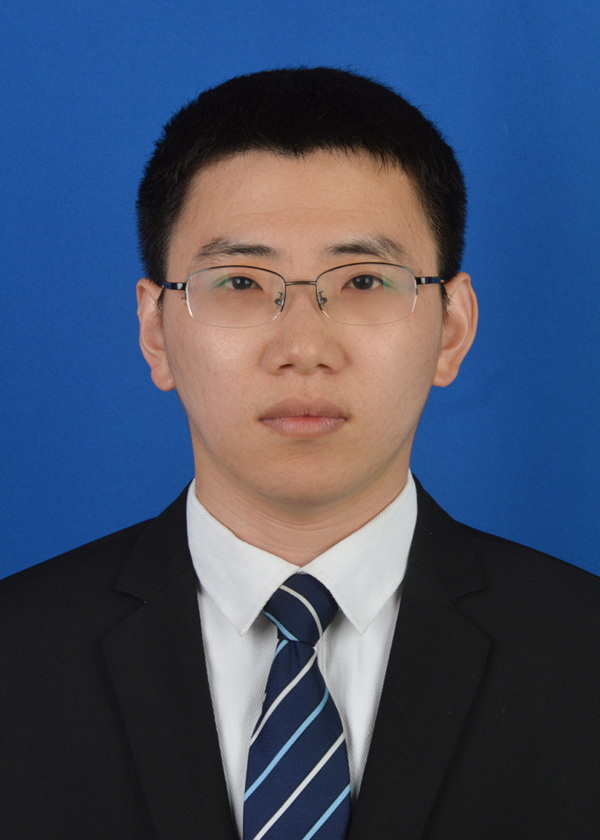
\includegraphics[width=1in,height=1.25in,clip,keepaspectratio]{figures/author/authorShanHe}}]{Shan He}
received the Ph.D. degree in control science and engineering from Nanjing
University of Science and Technology, Nanjing, China, in 2022.

He is currently an Associate Professor with the School of Automation, Nanjing
University of Science and Technology. His research interests include signal
processing and target tracking.
\end{IEEEbiography}

\begin{IEEEbiography}[{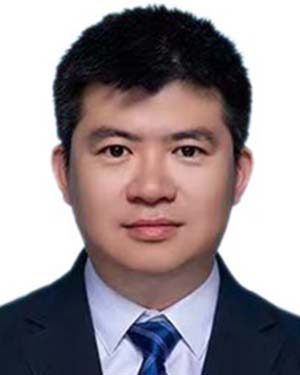
\includegraphics[width=1in,height=1.25in,clip,keepaspectratio]{figures/author/authorGuangyuanPan}}]{Guangyuan Pan}
(Member, IEEE) received the M.S. and Ph.D. degrees in control science and
engineering from Beijing University of Technology, Beijing, China, in 2012 and
2016, respectively, under Dr. Junfei Qiao's team.

From 2013 to 2014, he was a joint-training Ph.D. Student with the University of
Victoria, Victoria, BC, Canada. From 2016 to 2019, he was a Postdoctoral Researcher
with the Department of Civil and Environmental Engineering, University of Waterloo,
Waterloo, ON, Canada. From 2019 to 2020, he was a Research Associate with the
Department of Electronics and Electrical Engineering, The Chinese University of
Hong Kong, Hong Kong. He is now an Associate Professor with the Department of
Automation and Electrical Engineering, Linyi University, Linyi, China. His research
interests include machine learning and deep learning, data mining and signal
processing, transportation safety, and intelligent systems.
\end{IEEEbiography}

\end{document}
